% Independent XeLaTeX source. All observations are filled from audited files.
\documentclass[UTF8,a4paper,12pt]{ctexart}
\usepackage[left=23.5mm,right=23.5mm,top=22mm,bottom=22mm,headheight=15pt,headsep=6mm,footskip=10mm]{geometry}
\usepackage{amsmath,amssymb,booktabs,array,tabularx,tikz,xcolor,fancyhdr,hyperref,needspace}
\usetikzlibrary{arrows.meta}
\definecolor{ink}{gray}{0}
\definecolor{muted}{gray}{.26}
\definecolor{hair}{gray}{.62}
\definecolor{tint}{gray}{.96}
\hypersetup{hidelinks,
 pdftitle={变散热边界下离散温度场的残差误差上界},pdfauthor={徐楷沅 2352163},
 pdfsubject={人工智能与数学课程论文：自研残差上界研究智能体与温度误差估计}}
\IfFontExistsTF{STZhongsong}
  {\newCJKfontfamily\paperdisplay{STZhongsong}[FakeBold=1.7]}
  {\newcommand{\paperdisplay}{\bfseries}}
\IfFontExistsTF{Microsoft YaHei}
  {\newCJKfontfamily\paperlabel{Microsoft YaHei}[BoldFont={Microsoft YaHei Bold}]}
  {\newcommand{\paperlabel}{\sffamily}}
\newcommand{\runningface}{\normalfont\sffamily\paperlabel\fontsize{8.7}{10.6}\selectfont}
\pagestyle{fancy}\fancyhf{}
\fancyhead[L]{{\runningface\color{muted}变散热边界下离散温度场的残差误差上界}}
\fancyhead[R]{{\runningface\color{muted}人工智能与数学\enspace·\enspace 课程论文}}
\fancyfoot[L]{{\runningface\color{muted}徐楷沅\enspace{\color{hair}/}\enspace2352163}}
\fancyfoot[R]{{\runningface\color{ink}\bfseries\thepage}}
\renewcommand{\headrulewidth}{.4pt}
\renewcommand{\headrule}{{\color{hair}\hrule height\headrulewidth width\headwidth}}
\fancypagestyle{firstpage}{\fancyhf{}\renewcommand{\headrulewidth}{0pt}
  \fancyfoot[R]{{\runningface\color{ink}\bfseries\thepage}}}
\ctexset{section={format=\raggedright\normalfont\paperdisplay\fontsize{19}{24}\selectfont\color{ink},
 number={\normalfont\bfseries\arabic{section}},aftername=\hspace{.75em},
 beforeskip=1.65ex plus .35ex minus .2ex,afterskip=1.15ex plus .15ex},
 subsection={format=\raggedright\normalfont\bfseries\color{ink}\large}}
\newcommand{\papersectionbreak}{\par\addvspace{4.5mm}\Needspace{5\baselineskip}}
\newcommand{\para}[1]{\par\addvspace{.62\baselineskip}\noindent
  {\paperlabel\sffamily\bfseries\fontsize{10.7}{15}\selectfont\color{ink}#1}\hspace{.66em}\ignorespaces}
\newcommand{\resulthead}[2]{\par\addvspace{.7\baselineskip}\Needspace{4\baselineskip}\noindent
  {\sffamily\paperlabel\bfseries\fontsize{10.5}{15}\selectfont#1}\hspace{.82em}
  {\paperdisplay\fontsize{14}{19}\selectfont\color{ink}#2}\par\nobreak\vspace{.17\baselineskip}\noindent}
\newcommand{\prooflead}{\par\smallskip\noindent{\sffamily\paperlabel\bfseries\fontsize{10}{14}\selectfont\color{ink}证明}\hspace{.64em}}
\newcommand{\subhead}[1]{\par\addvspace{.87\baselineskip}\Needspace{3.2\baselineskip}\noindent
 {\paperlabel\sffamily\bfseries\fontsize{12.2}{17}\selectfont\color{ink}#1}\par\nobreak\vspace{.13\baselineskip}\noindent}
\newcommand{\source}[1]{\par\smallskip\noindent{\footnotesize\color{muted}#1}\par}
\newcommand{\capline}[2]{\par\noindent
 {\sffamily\paperlabel\bfseries\fontsize{9.6}{14}\selectfont#1}\hspace{.75em}
 {\sffamily\paperlabel\bfseries\fontsize{10.2}{15}\selectfont\color{ink}#2}\par\nobreak}
\newcommand{\norm}[1]{\left\lVert #1\right\rVert_\infty}
\newcommand{\one}{\boldsymbol 1}
\newcommand{\tabletype}{\linespread{1.06}\fontsize{10.5}{15.4}\selectfont\renewcommand{\arraystretch}{1.14}}
\newcommand{\columnhead}{\sffamily\paperlabel\bfseries\color{ink}}
\newcommand{\figurenote}[1]{\par\vspace{1.0mm}\noindent{\linespread{1.04}\fontsize{9.4}{14.7}\selectfont\color{muted}#1\par}}
\setlength{\parindent}{2em}\setlength{\parskip}{.18em plus .03em}
\setlength{\emergencystretch}{2em}
\setlength{\heavyrulewidth}{.7pt}\setlength{\lightrulewidth}{.35pt}
\setlength{\aboverulesep}{.55ex}\setlength{\belowrulesep}{.55ex}
\AtBeginDocument{\setlength{\abovedisplayskip}{7pt plus 2pt minus 1pt}
 \setlength{\belowdisplayskip}{7pt plus 2pt minus 1pt}
 \setlength{\abovedisplayshortskip}{4pt}\setlength{\belowdisplayshortskip}{4pt}}
\widowpenalty=8000 \clubpenalty=8000 \displaywidowpenalty=9000
\raggedbottom
\linespread{1.19}
\begin{document}
\thispagestyle{firstpage}
\noindent{\runningface 人工智能与数学\enspace·\enspace 课程论文}\hfill
{\normalfont\small\scshape Moonshine Thermal Lab}\par
\vspace{2mm}\noindent{\color{ink}\rule{\linewidth}{.55pt}}\par
\vspace{3.0mm}
\noindent\begin{minipage}[c]{.715\linewidth}
{\parindent=0pt\raggedright\color{ink}\paperdisplay\fontsize{26.4}{34}\selectfont
  变散热边界下离散温度场的\\残差误差上界\par}
\vspace{3mm}{\sffamily\paperlabel\fontsize{12.3}{17}\selectfont\color{muted}用自研数学智能体检验候选上界并寻找反例}\par
\vspace{3mm}{\sffamily\paperlabel\fontsize{10.2}{15}\selectfont 徐楷沅\quad{\color{muted}2352163}}\par
\end{minipage}\hfill
\begin{minipage}[c]{.26\linewidth}\centering
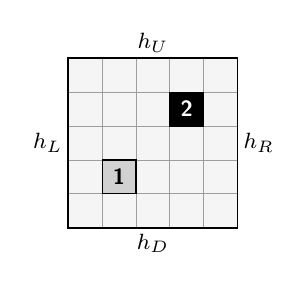
\begin{tikzpicture}[x=2.15cm,y=2.15cm,font=\fontsize{8.2}{10}\selectfont]
\fill[tint] (0,0) rectangle (1,1);
\draw[step=.2,color=hair,line width=.33pt] (0,0) grid (1,1);
\draw[ink,line width=.65pt] (0,0) rectangle (1,1);
\filldraw[fill=black!18,draw=ink,line width=.42pt] (.2,.2) rectangle (.4,.4);
\filldraw[fill=ink,draw=ink,line width=.42pt] (.6,.6) rectangle (.8,.8);
\node[ink,inner sep=0pt] at (.3,.3){\sffamily\bfseries 1};
\node[white,inner sep=0pt] at (.7,.7){\sffamily\bfseries 2};
\node[ink,above,inner sep=2pt] at (.5,1){$h_U$};
\node[ink,below,inner sep=2pt] at (.5,0){$h_D$};
\node[ink,left,inner sep=2pt] at (0,.5){$h_L$};
\node[ink,right,inner sep=2pt] at (1,.5){$h_R$};
\end{tikzpicture}\par\vspace{1mm}
{\sffamily\paperlabel\fontsize{8.3}{11}\selectfont\color{muted}方板上的热源强度与换热边界}\par
\end{minipage}\par
\vspace{2.2mm}
\noindent{\color{hair}\rule{\linewidth}{.45pt}}\par\vspace{1.0mm}
\noindent\begin{tabularx}{\linewidth}{@{}p{.105\linewidth}@{}X@{}}
{\sffamily\paperlabel\bfseries\fontsize{11}{16}\selectfont 摘\hspace{.26em}要} &
{\linespread{1.0}\fontsize{10.8}{16.4}\selectfont 我们开发了一个能用反例检验公式的数学研究智能体，用于判断快速求得的温度场何时可以接受。针对四边散热系数可变的离散导热模型，我们证明，保留残差的位置与正负可以收紧最大温度误差的上界。智能体由项目编写的精确检验器、研究控制器和模型接口组成，复用 Moonshine 分派工具。第一轮，@@LIVE_MODEL@@ Flash 请求检验一个允许正负残差直接抵消的简化式；检验器在第 @@LIVE_FIRST_N@@ 组发现它低估了误差。第二轮，模型依据回传的反例改查预设的双端点式，检验器查完 @@LIVE_SECOND_N@@ 组四格工况，域内未见反例。在三个大网格上，对同一批预测更换判据，报警由 @@OLDPAIRED@@ 次降为 @@NEWPAIRED@@ 次；各策略独立运行，完整重算由 @@OLDCLOSED@@ 次降为 @@NEWCLOSED@@ 次，本批总耗时未缩短。\par}\\[2.2mm]
{\sffamily\paperlabel\bfseries\fontsize{9.4}{14}\selectfont\color{muted}关键词} &
{\fontsize{9.6}{14.8}\selectfont\color{muted}数学研究智能体；反例检验；后验误差估计；离散导热；降阶模型}
\end{tabularx}\par\vspace{2.0mm}
\noindent{\color{hair}\rule{\linewidth}{.45pt}}\par\vspace{1.0mm}
%%PART problem
\section{问题与离散模型}
2026 年 6 月 1 日《EDA 专题第四期》第 4 页提出“热仿真加速”。本文选取其中的\href{https://github.com/orgyuanbao/MoonshineThermalLab/blob/ece5bbfffbbd722c43c94d691a0b714ffda7b0e5/MoonshineThermalLab/thermal/problem.md}{二维线性离散子问题}。四边换热强度改变后，降阶模型能快速给出一张新的温度图。若有公式保证每个格点的误差均小于容差，就可以接受预测，省去一次完整求解。困难在于，逐格的热量失衡可以直接计算，逐格的温度误差却依赖尚未知晓的完整解。本文研究能否利用热量失衡的幅度、位置与正负给出可靠上界，并开发一个智能体，在给定的工况中主动寻找足以推翻候选公式的反例。
\para{离散对象} 将单位方板分成 $n\times n$ 个等大控制体，边长 $\Delta=1/n$。导热系数为 1，环境温升为 0，两个方形热源 $[0.2,0.4]^2$ 和 $[0.6,0.8]^2$ 的源强分别为 1 和 2。载荷 $b$ 由热源与控制体交叠的面积积分得到。设 $K$ 为四邻接网格的图拉普拉斯，$D_s$ 标出边 $s$ 所接触的单元。角点累计两个边界面；若只有一个格子，则累计四个。离散温升 $T$ 满足
\begin{equation}
 A_\mu T=b,\qquad A_\mu=K+\sum_s\beta(h_s)D_s,\quad
 \beta(h)=\frac{\Delta}{1/h+\Delta/2},\qquad \mu\in[1/5,5]^4. \label{model}
\end{equation}
对预测 $\widehat T$，残差 $r=b-A_\mu\widehat T$ 与误差 $e=T-\widehat T$ 满足 $A_\mu e=r$。本文要估计的是相对离散真解的 $\norm e$。变 Robin 系数导热的降阶建模已有研究\cite{boyaval}，稀疏 $H$ 矩阵的分量误差估计亦有专门方法\cite{minamihata}。下文针对式~\eqref{model}，考察哪些残差信息会改变判据的实际决策。
%%PART bounds
\section{从逆矩阵的单调性得到逐格包络}
\para{两个比较算子} 记 $G_\mu=A_\mu^{-1}$。对于任意非零 $x$，$x^\top A_\mu x$ 是相邻单元差的平方和，加上非负的边界二次项。网格连通，所以它严格为正。若 $A_\mu x\ge0$ 而 $x$ 有负的最小值，最小点必须与所有邻点相等，否则该行的邻接差之和为负。沿网格传播到边界，边界项又严格为负，矛盾。于是 $G_\mu$ 逐项非负。
记 $G_w,G_s$ 分别为四边同时取最弱和最强散热时的逆。参数单调性给出 $A_\mu-A_w\ge0$、$A_s-A_\mu\ge0$，二者均为对角矩阵。恒等式
\[
 G_w-G_\mu=G_w(A_\mu-A_w)G_\mu,\qquad
 G_\mu-G_s=G_\mu(A_s-A_\mu)G_s
\]
将端点的参数序转为逐项的矩阵序 $0\le G_s\le G_\mu\le G_w$。

\resulthead{命题一}{最优统一倍数} 若只知道 $\norm r$，对全部许可参数和任意近似解都有效的最小常数是 $C_n^\star=\norm{G_w\one}$。\prooflead 逐项有 $|G_\mu r|\le\norm r\,G_w\one$。取弱边界及 $r=\one$ 即可达到等号；在给定 $b$ 的情况下，$\widehat T=G_w(b-\one)$ 产生的正是这个残差。早期由项目侧另行给出的屏障 $z_{ij}=[5+x_i(1-x_i)+y_j(1-y_j)]/(4\Delta^2)$ 满足 $A_\mu z\ge\one$，故原标量常数 $C_n^{\rm old}=\norm z\ge C_n^\star$。两者比较的是同一积分形式的单元残差。

\resulthead{命题二}{分块双端点界} 固定一个不相交的单元分块。对每块 $B$ 离线求 $W_B=G_w\one_B$ 和 $V_B=G_s\one_B$。在线读取 $\ell_B=\min_{j\in B}r_j$、$u_B=\max_{j\in B}r_j$，记 $t^+=\max(t,0)$、$t^-=\max(-t,0)$。令
\begin{equation}
 \begin{aligned} L&=\sum_B(\ell_B^+ V_B-\ell_B^-W_B),\\[-.1em]
 U&=\sum_B(u_B^+W_B-u_B^-V_B). \end{aligned} \label{interval}
\end{equation}
则 $L\le e\le U$。\prooflead 在每块上有 $\ell_B\one_B\le r\one_B\le u_B\one_B$，其中乘积按单元理解。施加非负矩阵 $G_\mu$ 后次序保持。正的上端点应乘较大的响应，负的上端点应乘较小的响应；对下端点反过来选取。利用 $V_B\le G_\mu\one_B\le W_B$ 并求和即得式~\eqref{interval}。

\para{三种信息量} 记 $p_B=u_B^+$，$q_B=\ell_B^-$，$m_B=\max(p_B,q_B)$。只用位置时取 $\eta_{\rm pos}=\norm{\sum m_BW_B}$；再区分正负时取 $\eta_{\pm}=\max\{\norm{\sum p_BW_B},\norm{\sum q_BW_B}\}$。完整包络的标量值为 $\eta_2=\max_i(U_i,-L_i)$。去掉式~\eqref{interval} 中由 $V_B$ 带来的抵消，再用 $p_B,q_B\le m_B\le\norm r$，得到
\begin{equation}
 \boxed{\;\norm e\le\eta_2\le\eta_\pm\le\eta_{\rm pos}\le C_n^\star\norm r\;} . \label{chain}
\end{equation}
仅保留 $m_B$ 时，在弱边界令每块残差恒为 $+m_B$ 即取到 $\eta_{\rm pos}$。这说明只凭这些块幅度不能再统一收紧。若细化块，子块极差收窄，且父块响应等于子块之和，故双端点区间只会缩小或保持。
\source{两份归档推导和相应的精确执行输出见 \hyperref[materials]{材料 B}。}
%%PART four_cell
\section{四格系统中可以精确看见的抵消}
四边均取 $h=1/5$ 时，$2\times2$ 网格的每格接触两个相同的外边界面。式~\eqref{model} 化为 $A=K+\tfrac4{21}I$。按下排从左到右、再按上排从左到右编号。下图的三个残差均满足 $\norm r=1$。统一倍数给出同一个上限；直接有理数消元和按模式的谱计算给出相同的逐例误差。
\par\medskip\noindent\begin{minipage}{\linewidth}\centering
@@MODE_PICTURE@@
\par\raggedright\vspace{2.4mm}
\capline{图 1}{三种残差排列以及各自的精确最大误差}
\figurenote{浅底格为 $+1$，深底格为 $-1$。每种排列均来自同一轮原生程序的输出（材料 C）。}\end{minipage}\par
\para{固定矩阵上的精确解} 取常量向量 $v_0$、两种方向的条纹 $v_1,v_2$ 和棋盘格 $v_3$，每个分量均为 $\pm1$。从格图计算得 $Kv_j=\lambda_jv_j$，其中 $\lambda_j$ 依次为 $0,2,2,4$。四个向量两两正交，故 $r=\sum_j a_jv_j$，$a_j=v_j^\top r/4$。于是
\[
 e=\sum_{j=0}^3\frac{a_j}{\lambda_j+4/21}\,v_j,\qquad
 \norm e\le\frac{21}{4}|a_0|+\frac{21}{46}(|a_1|+|a_2|)+\frac{21}{88}|a_3|.
\]
纯模式只有一项非零，所以图 1 的三个模态上界都取到等号。横条纹和棋盘格各有两正两负；横条纹的最大误差为棋盘格的 $@@STRIPE_RATIO@@$ 倍。棋盘格中的每条内边两端均异号，相邻传热对这种交替扰动的响应更小。这个对角化使用固定的四格矩阵，边界改变后需重新检验相应模式。
\para{一个会低估误差的替代式} 矩阵的逐项序只保证对非负载荷的比较。在前期原版 Moonshine 的第二轮推导中，取 $r=@@COUNTER_R@@$，右边界调为 $5$，其余仍为 $1/5$。用弱边界直接乘这个带符号向量，会低估真实误差：
\[
  \underbrace{\norm{G_w r}}_{\text{替代式给出的值}}=@@UNSAFE@@
  \;<\;@@ACTUAL@@=\underbrace{\norm{G_\mu r}}_{\text{真实最大误差}} .
\]
弱边界作用于正负两部时各自增大，两者的差却未必增大，因此这种替代式不能作为安全判据。
\para{核对范围} 独立有理数程序还在 @@NUM_PARAMS@@ 组边界、@@PATTERNS@@ 个三值残差上检查嵌套分块，共含 @@EXACT_PAIRS@@ 个边界与残差组合。有限穷举帮助发现实现错误；连续参数区间的覆盖见式~\eqref{interval} 的证明。
%%PART research
\section{前期推导与原版 Moonshine 的检验记录}
\par\medskip\noindent\begin{minipage}{\linewidth}\capline{表 1}{原生研究记录中的早期七轮}
\vspace{2mm}\tabletype\renewcommand{\arraystretch}{1.30}
\begin{tabularx}{\linewidth}{@{}lXrrr@{}}\toprule
{\columnhead 轮次} & \multicolumn{1}{l}{\columnhead 本轮实际推进的内容} & {\columnhead Python 成功/尝试} & {\columnhead 审核通过/尝试} & {\columnhead 归档条目}\\\midrule
@@HISTORY_ROWS@@
\bottomrule\end{tabularx}
\figurenote{表中计数来自工具回执；一次审核可分派若干审核角色，一次程序执行也可覆盖多个工况。表内合计 @@HIST_SUCCESS@@ 次成功执行、@@HIST_REVIEW@@ 次审核通过及 @@HIST_ARCHIVE@@ 条归档。}\end{minipage}\par
\subhead{前期单端界检验} 我们给出模型、参数范围和“能否利用位置与正负”的问题，允许分块，起初未指定公式。原版 Moonshine 通过本机 Codex 适配器调用 \texttt{@@MODEL@@}，推导单端符号界并编写分数检验程序。在 @@FIRST_TOTAL@@ 个工况中，@@FIRST_GAIN@@ 个上界严格小于统一标量界。首次整体审核因证据不足暂未得出结论。计算审核者当时收到 @@REVIEW_SMALL@@ 字符的材料；补交脚本和输出后，材料增至 @@REVIEW_LARGE@@ 字符，复审通过。
\subhead{前期双端界检验} 我们随后提供双端点候选式，请原版 Moonshine 沿用上述模型检验符号方向和比较条件。它编写程序，枚举 @@SECOND_TOTAL@@ 个参数、残差和分块组合，其中 @@SECOND_GAIN@@ 个双端界严格紧于单端符号界。上一节右边界加强的反例来自这次检验。以下第~\ref{extension}~节另行记录自研智能体接入 @@LIVE_MODEL@@ Flash 后完成的两轮在线实验。
\subhead{四格示例与报告生成} 对固定四格矩阵和三种残差排列，原版 Moonshine 在一次专门会话中补全条纹模态、运行有理数程序，并保存推导、计算输出和审核记录。我们为这些材料编写了 LaTeX 报告技能，图 1 的三个精确值可以逐项核对。生成本文时，该技能还读取前期研究、自研智能体的回执和独立运行的大网格数据。报告生成发生在研究结束后，各轮审核针对当轮的推导和计算。
\source{早期各轮详见 \hyperref[materials]{材料 A}；两轮符号界的初审、复审、证明及程序结果详见材料 B；四格专轮详见材料 C。}
%%PART agent_extension
\clearpage
\section{自研残差上界研究智能体}\label{extension}
要判断公式声称的上界是否安全，只需找到一组“实际误差大于上界”的输入，就能否定猜想。我们据此开发了残差上界研究智能体（Residual Bound Agent）。研究者提供候选公式、枚举范围和换式条件；智能体把一次检验得到的精确反例或覆盖数交还模型，让下一步决定有可复算的依据。

\para{精确检验器} 我们在 \texttt{residual\_tool.py} 中复用四格系统的有理数求逆与分块计算，实现工具 \texttt{check\_residual\_bound}。输入是候选界 $H$、分块、缩放倍数和枚举域。程序逐组比较 $\norm{G_\mu r}$ 与 $H(r,\mu)$；若发现低估，就返回首个反例的边界、残差、误差向量和两个精确值，否则返回实际检查数和总数。

\para{研究控制器} 我们在 \texttt{bound\_agent.py} 中实现了检查、反馈和停止规则。控制器接收模型的 \texttt{check} 或 \texttt{finish} 动作，核对参数和轮数预算，并识别重复请求。我们将检验器注册到 Moonshine 的 \texttt{ToolManager}，由它分派每次检验。工具返回后，控制器核验回执并更新历史，运行入口将已完成的步骤写盘。

\para{模型接口} 我们编写 \texttt{bound\_agent\_model.py}，通过@@LIVE_PROVIDER@@接入 @@LIVE_MODEL@@ Flash，请求标识为 \texttt{deepseek-v4.1-flash}，公开实验记录简称“@@LIVE_MODEL@@”。接口把研究目标和工具定义发给模型，将上一轮的工具结果与调用标识配对，供模型继续请求检验或提交结束说明。
\par\medskip\noindent\begin{minipage}{\linewidth}\centering
\begin{tikzpicture}[
 x=1cm,y=1cm,
 actor/.style={draw=ink,fill=white,line width=.54pt,minimum width=4.28cm,minimum height=1.07cm,align=center,inner sep=3pt,font=\small},
 ours/.style={actor,fill=tint,line width=.85pt},
 link/.style={-{Stealth[length=2.1mm,width=1.35mm]},line width=.65pt,draw=ink},
 labeltext/.style={font=\footnotesize\paperlabel,fill=white,inner sep=1.6pt}]
\node[actor] (task) at (0,0) {\textbf{研究者}\\给定候选式与切换条件};
\node[actor] (model) at (5.15,0) {\textbf{@@LIVE_MODEL@@ Flash}\\选择检验或结束};
\node[ours] (control) at (10.30,0) {\textbf{自研控制器}\\核对行动与轮数预算};
\node[actor] (moon) at (10.30,-2.70) {\textbf{Moonshine 工具管理器}\\按已注册的定义分派调用};
\node[ours] (tool) at (5.15,-2.70) {\textbf{自研精确检验工具}\\有理数枚举并产生结果};
\node[ours] (record) at (0,-2.70) {\textbf{自研控制器与适配器}\\核验、保存并回传结果};
\node[draw=ink,fill=tint,rounded corners=2mm,inner xsep=4mm,inner ysep=1.4mm,font=\small] (stop) at (5.15,1.53) {自研控制器保存结束结论};
\draw[link] (task.east)--(model.west);
\draw[link] (model.east)--node[midway,above,font=\scriptsize]{检验}(control.west);
\draw[link] (model.north)--node[midway,right,labeltext]{结束}(stop.south);
\draw[link] (control.south)--(moon.north);
\draw[link] (moon.west)--(tool.east);
\draw[link] (tool.west)--(record.east);
\draw[link] (record.north)--(0,-1.35)--node[midway,above,labeltext]{反例或检查数}(5.15,-1.35)--(model.south);
\end{tikzpicture}
\par\raggedright\vspace{2mm}\capline{图 2}{模型选择检验，自研程序计算并回传结果}
\figurenote{浅灰框为项目实现。第一份回执给出第 @@LIVE_FIRST_N@@ 个工况的反例，第二份给出 @@LIVE_SECOND_N@@ 个工况的检查结果。Moonshine 分派两次工具调用，精确求解均由同一个本地检验器完成。}\end{minipage}\par

\source{开发所用的控制器、模型适配器、数学工具与校验用例见 \hyperref[materials]{材料 E、G}。}

\clearpage
\subsection*{两轮在线实验：由反例触发第二次检验}
我们把两条候选式和一个条件交给模型：先检验把带符号残差整体代入弱散热端点的简化式，若发现反例，就在同一域内检验式~\eqref{interval} 的双端点界。两条候选式及切换条件由研究者给定。模型需要读取实际回执，决定何时请求下一次检验、何时结束。

\subhead{第一轮：简化式在哪一组工况低估了误差？}
DeepSeek 请求检验 \texttt{weak\_signed}，即以 $H_0(r)=\norm{G_w r}$ 估计 $\norm{G_\mu r}$。这个简化式允许正负项先抵消，与式~\eqref{chain} 中分别估计两者的 $\eta_\pm$ 不同。自研控制器接受请求，Moonshine 把它分派给已注册的检验器。检验器在第 @@LIVE_FIRST_N@@ 组首次发现低估。按左、右、下、上的边界次序和先下排后上排的单元编号，输入为
\[
   (h_L,h_R,h_D,h_U)=@@LIVE_H@@,\qquad r=@@LIVE_R@@^\top .
\]
即上边散热强、其余三边弱，上排两格残差为正、下排两格为负。本地有理数求解给出
\[
    \underbrace{@@LIVE_ERROR@@}_{\text{真实误差 }\norm{G_\mu r}}
       -\underbrace{@@LIVE_BOUND@@}_{\text{候选上界 }H_0(r)}=@@LIVE_GAP@@>0 .
\]
公式声称误差至多约 $0.457$，实际却约为 $0.742$。这一个工况即推翻了简化式。控制器保存反例，模型接口把输入、两个分数和已查组数一并送回 DeepSeek。

\subhead{第二轮：保持检验条件，换用分块双端点式}
DeepSeek 读到反例后按约定发起第二次检验。两轮之间无需研究者修改程序，模型仅更换候选参数：
\begin{center}\ttfamily\small \{"candidate": "block\_two\_endpoint"\}\end{center}
\noindent Moonshine 将请求分派给同一个检验器，网格、单格分块和缩放倍数 $1$ 均保持不变。每条边有两种取值，四条边共 $2^4=16$ 种组合；每格残差取 $-1,0,1$，四格共 $3^4=81$ 种组合。检验器逐一比较真实误差与 $\eta_2$，全部 $16\times81=@@LIVE_SECOND_N@@$ 组均未发现低估。

\para{何时停止} 自研控制器记录完整覆盖数并将结果回传。DeepSeek 据此选择 \texttt{finish}，回答中明确了有限枚举的范围：
\begin{quote}\small @@LIVE_FINISH_EXCERPT@@\end{quote}
\noindent 实验留下两次检验动作及一次结束动作。在连续边界参数盒 $[1/5,5]^4$ 上，双端点界成立的依据是命题二的逐项比较证明。
\source{原始任务、模型选择的参数、逐轮有理数结果与结束答复均见 \hyperref[materials]{材料 F}。所附复核程序可在本机重新计算两轮数学结果。}

\clearpage
\subsection*{开发验证与独立的本地策略试验}
\para{从数学工具查到模型接口} 我们将反例中的边界和误差向量代回 $A_\mu e$，逐格核对输入残差；再让一份只检查过一组却声称“搜索完毕”的回执进入控制器，确认程序会停止并保留已验证步骤。模型接口测试则由本机模拟服务应答 @@HTTP_REQUESTS@@ 次 HTTP 交互，检查请求标识与结果的配对。前节的两轮研究使用真实的@@LIVE_PROVIDER@@模型接口，归档中的两个工具结果也可以离线逐项复算。

\para{让运行可以中断和复核} 在交互入口，每完成一次数学检验，程序先写入临时文件，再替换本轮的 JSON 记录。这样，即使在下一次响应到来前按下中断键，已经完成的轮次仍可查看。记录包含目标、模型选过的参数、工具返回值与结束原因。报告技能在事后读取这些材料生成论文。

\para{用另一种策略单独检查停止规则} 直接运行 \texttt{python thermal\_agent.py investigate} 会使用项目编写的本地策略。在默认域中，四边各取 $\{1/5,5\}$，四格残差各取 $\{-1,0,1\}$，共有 $2^4\,3^4=1296$ 组。该策略遇到反例后选择修正式，再由已知可行倍数与见证给出的下限选择下一次缩放倍数。表 2 记录这次独立运行。

\par\medskip\noindent\begin{minipage}{\linewidth}\capline{表 2}{本地策略的三轮精确检验（模型调用 @@TOOL_MODEL_CALLS@@ 次）}
\vspace{2mm}\tabletype
\begin{tabular*}{\linewidth}{@{}c@{\extracolsep{\fill}}lrrl@{}}
\toprule {\columnhead 次序}&{\columnhead 候选式}&{\columnhead 实查}&{\columnhead 域内总数}&{\columnhead 结果}\\\midrule
@@TOOL_STEPS@@
\bottomrule\end{tabular*}\end{minipage}\par

\para{能否再乘一个小于 1 的常数？} 本地策略第三次调用将双端点上界乘以 $@@SCALE_FACTOR@@$。在四边均取弱端点、$r=@@SCALE_R@@^\top$ 时，实测 $\norm e=@@SCALE_ERROR@@$，缩放上界仅为 $@@SCALE_BOUND@@$。由这一见证反推，原双端点上界在此例恰好等于真实误差。因此对本模型的单格分块，统一下调所有工况的倍数会失效；其他工况仍可有余量。
\source{本地策略的数学结果见 \hyperref[materials]{材料 E}，写盘、异常处理与测试入口见材料 G。}
%%PART experiments
\clearpage
\section{大网格实验：两种问题，两组计数}
采用 $@@GRID_STRING@@$ 三种网格。每种网格内，五种策略共用该网格的八维 POD 初始基 $V$，以 $V^\top A_\mu V y=V^\top b$ 得到预测 $Vy$。训练参数 24 组、调参参数 12 组，三个网格复用同一批参数，在 @@QUERIES@@ 组冻结散热参数上测试。每块板固定分成 $@@PARTITION@@$ 个空间块，容许的无量纲温升误差为 $\tau=@@TOL@@$。若判据大于阈值，则执行完整求解；自适应策略用这个新解增广基。事后完整参照解只用于计算真实误差。
\para{配对诊断} 保留旧策略每次回退前的预测，逐一替换五种界。预测及其真实误差固定，所以报警数的变化只反映证书提供的信息。另保留固定八维基的整条预测轨迹用于考察保守性。
\para{独立部署} 各策略从相同初始基出发独立决定是否回退，后续基底和预测可能分化。实验共记录 @@PAIRED_ROWS@@ 条配对预测行、@@CLOSED_ROWS@@ 条独立部署行；前者每行含五种界，后者每行只对应一种策略。
\par\medskip\noindent\begin{minipage}{\linewidth}\capline{表 3}{原参数流的报警与回退次数}
\vspace{2mm}\tabletype\begin{tabular*}{\linewidth}{@{}l@{\extracolsep{\fill}}rrr@{\hspace{6mm}}rrr@{}}\toprule
 & \multicolumn{3}{c}{\columnhead 固定旧轨迹：报警} & \multicolumn{3}{c}{\columnhead 各策略部署：回退}\\
\cmidrule(lr){2-4}\cmidrule(lr){5-7}判据 & @@GRID_HEADS@@ & @@GRID_HEADS@@\\\midrule
@@DECISION_ROWS@@
\bottomrule\end{tabular*}\end{minipage}\par\smallskip
旧轨迹对照中，新界令报警减少 @@PAIRED_SAVED@@ 次。策略独立学习后，实际少做 @@CLOSED_SAVED@@ 次完整求解。初期增广一次基会改变多个后续工况，因此不能用一组计数替代另一组。
\para{一次恰好改变决定的预测} 第 @@CASE_I@@ 次 $@@CASE_N@@^2$ 网格预测的四边系数为\par\centerline{$(h_L,h_R,h_D,h_U)=(@@CASE_MU@@)$。}
\noindent 图 3 将两个上界除以阈值；原值分别为 $@@CASE_POS@@$ 和 $@@CASE_SIGN@@$。同一行的完整参照解给出最大误差约为 $@@CASE_TRUE@@$。
\par\medskip\noindent\begin{minipage}{\linewidth}\centering @@CASE_CHART@@\par\raggedright\vspace{2.2mm}
\capline{图 3}{空间上界刚越过阈值，正负分离后可直接接受}
\source{逐次数据、参数和计时口径见 \hyperref[materials]{材料 D}。}\end{minipage}\par
%%PART discussion
\clearpage
\section{代价、适用范围与结论}
\para{哪些预测仍然难以判断？} 在固定八维基上，三个网格分别只有 @@FIXED_EX@@ 个真实超标工况，但每种判据仍对每个网格的全部 @@QUERIES@@ 个预测报警。双端点界与原标量界的逐例比值中位数分别为 @@FIXED_RATIOS@@。即使上界大幅缩小，仍可能高于决策阈值。在两种轨迹的全部 @@PAIRED_ROWS@@ 条预测中，双端点界与单端符号界@@EQUIV@@。式~\eqref{interval} 中，一个块只有在全部残差严格同号时，才可能提供非零的强端点修正。这解释了为何小网格有严格改进而大网格可以相等。
\par\medskip\noindent\begin{minipage}{\linewidth}\capline{表 4}{训练至返回结果的完整部署耗时（秒）}
\vspace{2mm}\tabletype\renewcommand{\arraystretch}{1.31}\begin{tabular*}{\linewidth}{@{}l@{\extracolsep{\fill}}rrrr@{}}\toprule
{\columnhead 网格} & {\columnhead 原标量} & {\columnhead 单端符号} & {\columnhead 双端点} & {\columnhead 双端点模板存储（MiB）}\\\midrule
@@COST_ROWS@@
\bottomrule\end{tabular*}
\figurenote{每格是 @@REPEATS@@ 次本机归档计时的中位数，含训练、模板准备、预测、回退和更新。参照误差复核与模型研究时间另计。模板栏按两组响应向量的字节数计算。}\end{minipage}\par
\subhead{独立参数流} 保持相同训练集和策略定义，在 $@@FRESH_N@@^2$ 网格另抽 @@FRESH_NQ@@ 组系数（种子 @@SEED@@），与原序列、训练集和调参集的重合数为 @@OVERLAP@@。原标量回退 @@FRESH_OLD@@ 次，双端点回退 @@FRESH_NEW@@ 次；双端点纠正了 @@FRESH_PRE@@ 次真实超标，返回结果超标 @@FRESH_RETURN@@ 次。冻结旧流各策略的返回超标合计为 @@RETURN_EX@@。这两条流评价了观测到的工况，全参数保证仍依靠证明。
\subhead{使用边界} $K_b$ 个块需要 $2K_b$ 张端点响应图，每张含 $n^2$ 个分量。可在两次矩阵分解后批量求离线响应，在线直接组合的工作量为 $O(K_b n^2)$。表 4 中，双端点策略虽减少回退，完整执行时间在本次三个网格上均高于旧标量策略。耗时受实现和机器负载影响。
\subhead{结论} 在变散热边界的离散系统中，保留残差的分块位置与正负可收紧温度误差上界。我们开发的智能体以四格精确反例否定了允许正负直接抵消的简化式，并将反例交给 DeepSeek；模型按预设条件转入双端检验。命题二给出整个参数盒上的数学保证。大网格上，改用新界使固定预测少报 @@PAIRED_SAVED@@ 次警，独立运行少做 @@CLOSED_SAVED@@ 次完整求解，现有实现的总耗时仍较长。上述估计针对离散模型；大网格浮点计算未作有向舍入，连续方程的离散化误差另需估计。

若只允许存储 $2K_b$ 张响应图，怎样选取 $K_b$ 个块以最小化回退和在线求值的总成本？本文固定采用同一分块，尚未求解这个优化问题。后续可以在训练工况上选块，再由独立参数流评价。
%%PART sources
\clearpage
\section{复核材料与文献}\label{materials}
材料 B 和 C 保存原生推导，D 保存大网格逐次结果。E、F 分别记录本地策略和真实模型会话，G 列出开发时的运行入口与测试。论文表格从归档取值。
@@SOURCE_LIST@@
\subhead{复算入口} 下面的命令在 \texttt{MoonshineThermalLab} 子目录运行。自研智能体的回放读取已归档的模型动作，本地重新计算两次工具结果并核对回执，无须连接模型服务。
\par\smallskip\noindent
\begin{tabular}{@{}l@{\hspace{5mm}}l@{}}
{\footnotesize\paperlabel\color{muted}自研两轮复算} & \texttt{\small python residual\_study/agent\_extension/verify\_live\_trace.py}\\
{\footnotesize\paperlabel\color{muted}四格示例复算} & \texttt{\small python report\_example/verify.py}\\
{\footnotesize\paperlabel\color{muted}原生程序复放} & \texttt{\small python residual\_study/moonshine/replay.py}\\
{\footnotesize\paperlabel\color{muted}大网格复算} & \texttt{\small python residual\_study/run\_experiment.py}
\end{tabular}
\figurenote{大网格复算可附加 \texttt{-{}-check-against residual\_study/results}，逐行比对冻结记录。}
\begin{thebibliography}{9}\fontsize{10.1}{15.2}\selectfont\setlength{\itemsep}{.55em}
\bibitem{boyaval} S. Boyaval, C. Le Bris, Y. Maday, N. C. Nguyen, A. T. Patera.
A reduced basis approach for variational problems with stochastic parameters: Application to heat conduction with variable Robin coefficient.
\textit{Computer Methods in Applied Mechanics and Engineering}, 198 (2009), 3187--3206.
\href{https://doi.org/10.1016/j.cma.2009.05.019}{出版记录}.
\bibitem{minamihata} A. Minamihata, K. Sekine, T. Ogita, S. M. Rump, S. Oishi.
Improved error bounds for linear systems with $H$-matrices.
\textit{Nonlinear Theory and Its Applications, IEICE}, 6 (2015), 377--382.
\href{https://doi.org/10.1587/nolta.6.377}{出版记录}.
\end{thebibliography}
